\chapter{Mapping}
A mapping campaign is planned in the experimental hall, where the n2EDM experiment is going to be located. There are numerous magnetic sources in the vicinity of the site, causing the magnetic environment to be unusually complex. Taking a number of magnetic field maps will provide knowledge necessary to make sure, that the n2EDM compensation system will be able to cope with the environment. A 2.5m high mobile tower with 10 3-axis magnetic field sensors has been constructed. The position and orientation of the tower is measured with cable extension transducers, which makes the mapping process as simple as sweeping an area with the tower. Reproducibility of the maps measured with the device was proven to be better than \SI{0.5}{\micro\tesla}.


\section{The idea}
The precision is not crucial, but the time it takes to measure a map is. The shorter it takes to make a map, the less it is influenced by external conditions. It cannot always be mapped during ,,quiet periods''. We want to have maps of magnetic fields that occur only during busy day-times. For example the crane, or SULTAN or other magnets.

For these reasons it has been decided, that the mapping would consist of a tower. The tower would be moved manually (don't use the future tense here), the position and orientation measured along the magnetic field. Then describe the setup here, briefely. The scalar information is enough to localise sources of magnetic field.

Vector information is useful if the data are to be used for example to calculate dedicated compensation coils for some sources of disturbance.

The setup is shown\ldots The mapper was a tower this and that high, with ten fluxgate magnetometers mounted on it.
The three analogue string potentiometers were mounted on a rigid L-piece. The base element is the string potentiometer. It consists of a wire wound on a spring-loaded spool, the spool attached to a potentiometer. For maximal linearity it is constructed in a way, that the string is wound one in layer only. The string string potentiometers give an analogue signal proportional to the extension of the wire. This information was used to determine the position and orientation of the tower.
\marginpar{Other names for a string potentiometers include: cable-extension transducer, draw-wire sensor and string pot.}
\mnote{The terms like the tower need to be clear by here.}


Let us start with a two-dimensional problem. Span two strings between a magnetic field sensor, each to a fixed position in the room. Based on trilateration. With two strings there are two solutions, but we are always able to detect the correct one.

To get the vector information about the field, also the orientation of the sensors needs to be known. For that an arm can attached to the sensor and a third string spanned to the arm's end.

Now is the time for the nice drawing of the geometry solution.



\section{Principle of a string-potentiometer--based mapper}
For a given signal of a calibrated string potentiometer the points where the free end of the string can be make up a circle. The centre at the location of the body of the sensor, the radius equal to the extension of the wire. In the mapper setup there are two string potentiometers mounted on the fixed L-piece, both extended to a single point on the tower. This points lies on the intersection of the two circles. The problem of determining the location based on the measurement of the distances to a set of fixed points is called \emph{trilateration}.

\marginpar{Other position determination methods include triangulation (measurement of angles between lines connecting a set of fixed points) and multilateration (measurement of the differences of distances between a set of fixed points).}

\begin{figure}
  \centering
  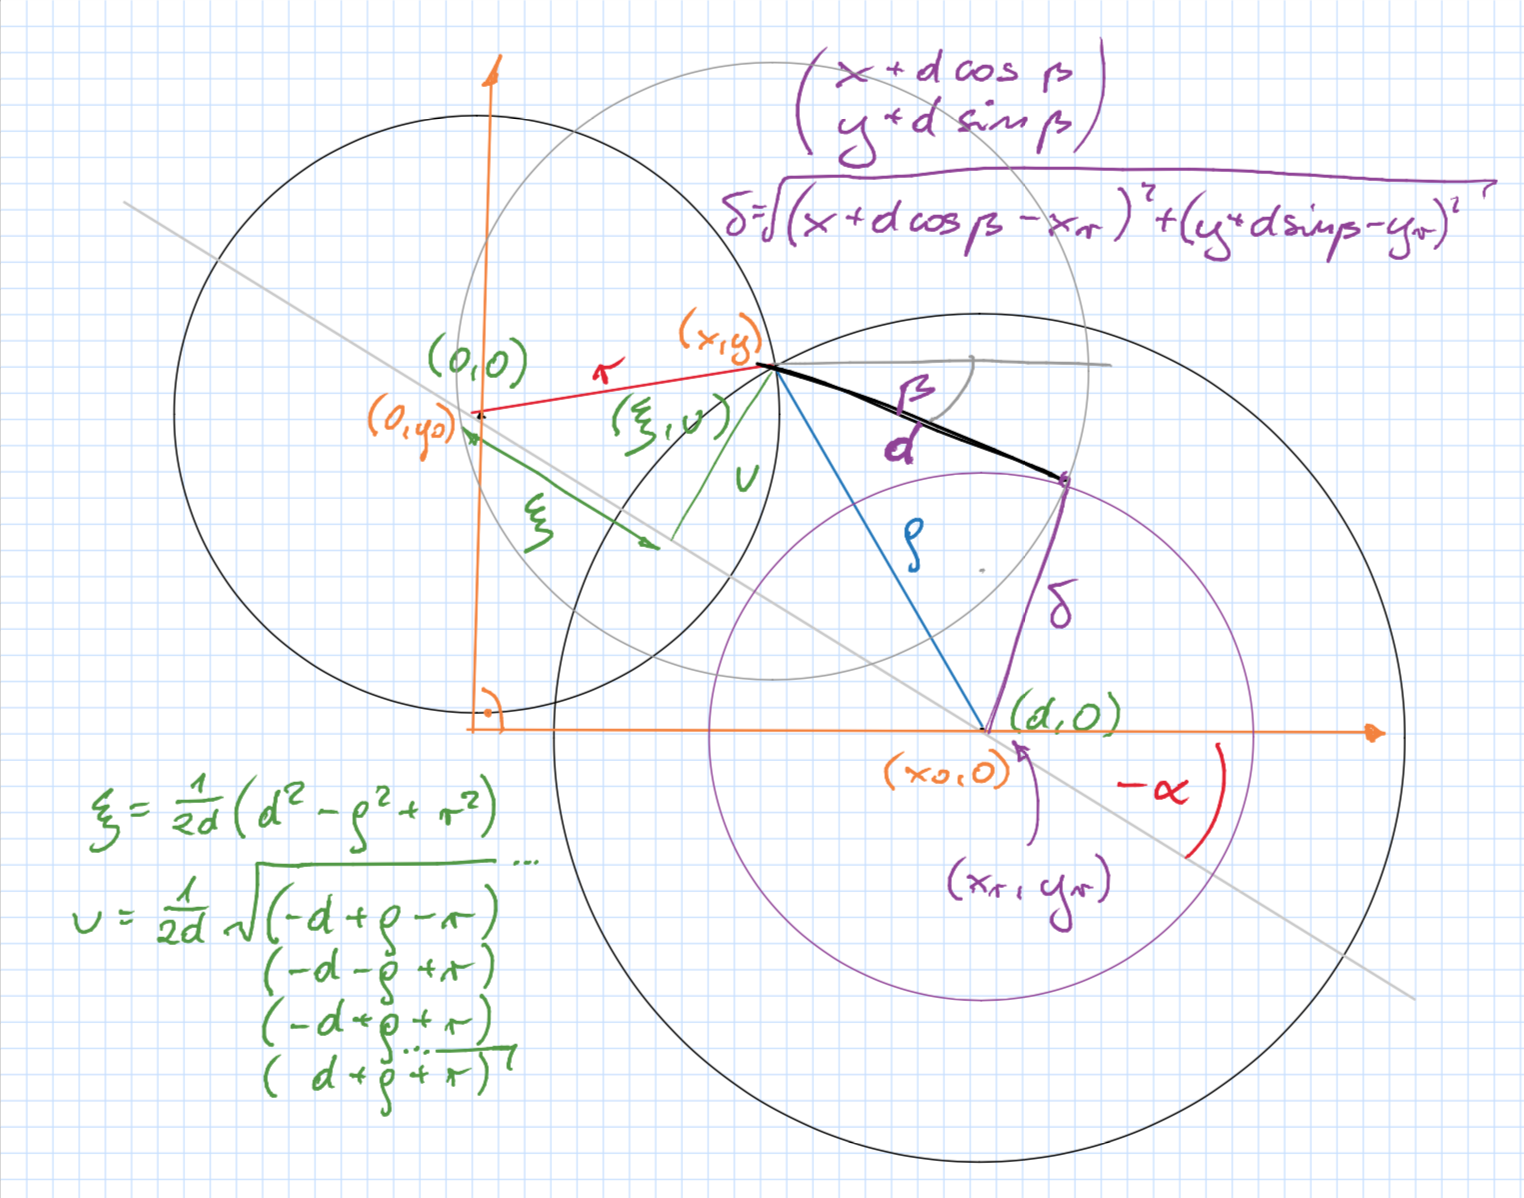
\includegraphics[width=0.9\linewidth]{gfx/mapping/geometry.png}
  \caption{\ldots}
  \label{fig:mapping_geometry}
\end{figure}

The geometry is presented in Fig.\,\ref{fig:mapping_geometry}.The two string potentiometers used to determine the position are located is points $(x, y) = (0, y_0)$ and $(x_0, 0)$ (in the L-piece coordinate system, orange in the figure).
The tower, here point-like, is at $(x,y)$.
The wire extensions are $r$ and $\rho$. For the sake of simplicity, we first give the solution in the coordinate system depicted in green \note{maybe use the A B and C names here already}, where the first string potentiometer is in $(0,0)$ and the second in $(d, 0)$ (with $d = \sqrt{x_0^2 + y_0^2}$). In this coordinate system the tower is in $(\xi, \nu)$. From simple geometry the solution for the position of the tower is:
\begin{align}
  \xi & = \frac{1}{2d} \left( d^2 - \rho^2 + r^2 \right) \\
  \nu & = \frac{1}{2d} \sqrt{ (-d + \rho - r) (-d - \rho + r) (-d + \rho + r) (d + \rho + r) }
\end{align}
The transformation to the L-piece, orange, coordinate system is rotation by the angle $\alpha = \mathrm{ctan} \frac{y_0}{x_0}$ followed by a translation:
\begin{equation}
  \begin{pmatrix}
    x \\
    y
  \end{pmatrix}
  =
  \begin{pmatrix}
    \cos \alpha & -\sin \alpha \\
    \sin \alpha & \cos \alpha
  \end{pmatrix}
  \begin{pmatrix}
    \xi \\
    \nu
  \end{pmatrix}
  +
  \begin{pmatrix}
    0 \\
    y_0
  \end{pmatrix}
\end{equation}

\note{Give here a general formula for an intersection of two circles. Need to check the LabVIEW code?}

With two circles there are two solutions, symmetric around the line connecting the centres of the circles. However, during the mapping the tower stays in the area inside the positive quarter of the L-piece coordinate system.
We assume never to be in the small triangle to the left and down from the line connecting the two string potentiometers.

The problem of determining the orientation of the tower is, in fact, the same as the one of the position. The setup includes a third string potentiometer, with the string attached to \note{there are two $d$s in the picture!} an arm of the tower (depicted in violet in Fig.\,\ref{fig:mapping_geometry}) of the length $a$. The end of the arm lies on the intersection of two circles: the one centred in the centre of the tower and radius $a$, and the one centred at the sensor end of the third potentiometer with the length equal to the wire extension.

Comment on the sensitivity here. The solution is best conditioned, when the angle of the intersection of the circles is large. There is a problem, in particular, in the ,,upper-left corner''.



\section{LPSC campaign}
The mapper setup was used to perform a mapping of the magnetic field performed in Laboratoire de Physique Subatomique \& Cosmologie (LPSC) in Grenoble, France in the days 6.-10.03.2017, with the much appreciated help of Rémi Faure, Guillaume Pignol and Dominique Rebreyend. The goal was to map two rooms, referred to as \emph{Bastille} and \emph{Chalet}. The rooms were considered to host a magnetic-field sensitive setup for Hg-199 magnetometry. In particular, gradients above roughly \SI[per-mode=symbol]{10}{\nano\tesla\per\centi\meter} cause an increase in the depolarisation rate of the mercury atoms.

\begin{figure}
  \centering
  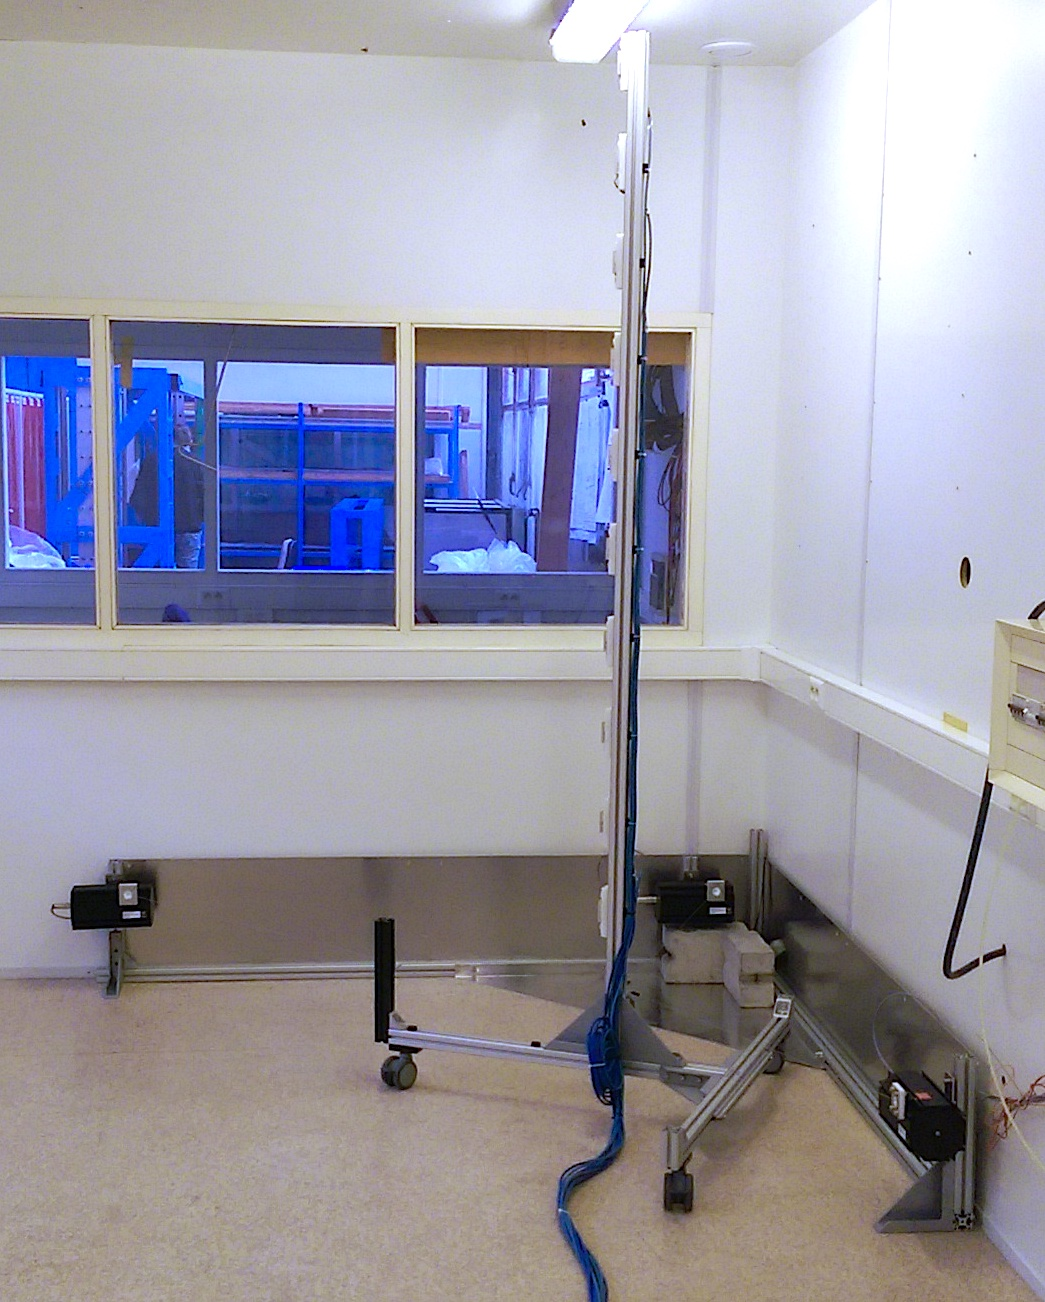
\includegraphics[width=0.9\linewidth]{gfx/mapping/lpsc/setup_edited.jpg}
  \caption{\ldots}
  \label{fig:mapping_bastille_setup}
\end{figure}

A photograph of the mapping setup is shown in Fig.\,\ref{fig:mapping_bastille_setup}. The movable \SI{2.5}{\meter} high tower was equipped with ten 3-axis fluxgate magnetic field sensors. The stationary coordinate system featured three string potentiometers spanned to the tower. The string pots were equipped with a custom made attachments that allowed the string to come at an angle out of the device. Two of the strings were attached to a point where the vertical beam with the fluxgates is, the third (left on the picture) was attached to the black, short vertical profile on the tower.

\marginpar{Technical details of the setup: fluxgates -- Stefan-Mayer FLC3-70, ADC -- aoethu, string potentiometers -- Micro-Eplison WDS-15000-P115-SA-P, readout frequency -- xxx}

\begin{figure}
  \centering
  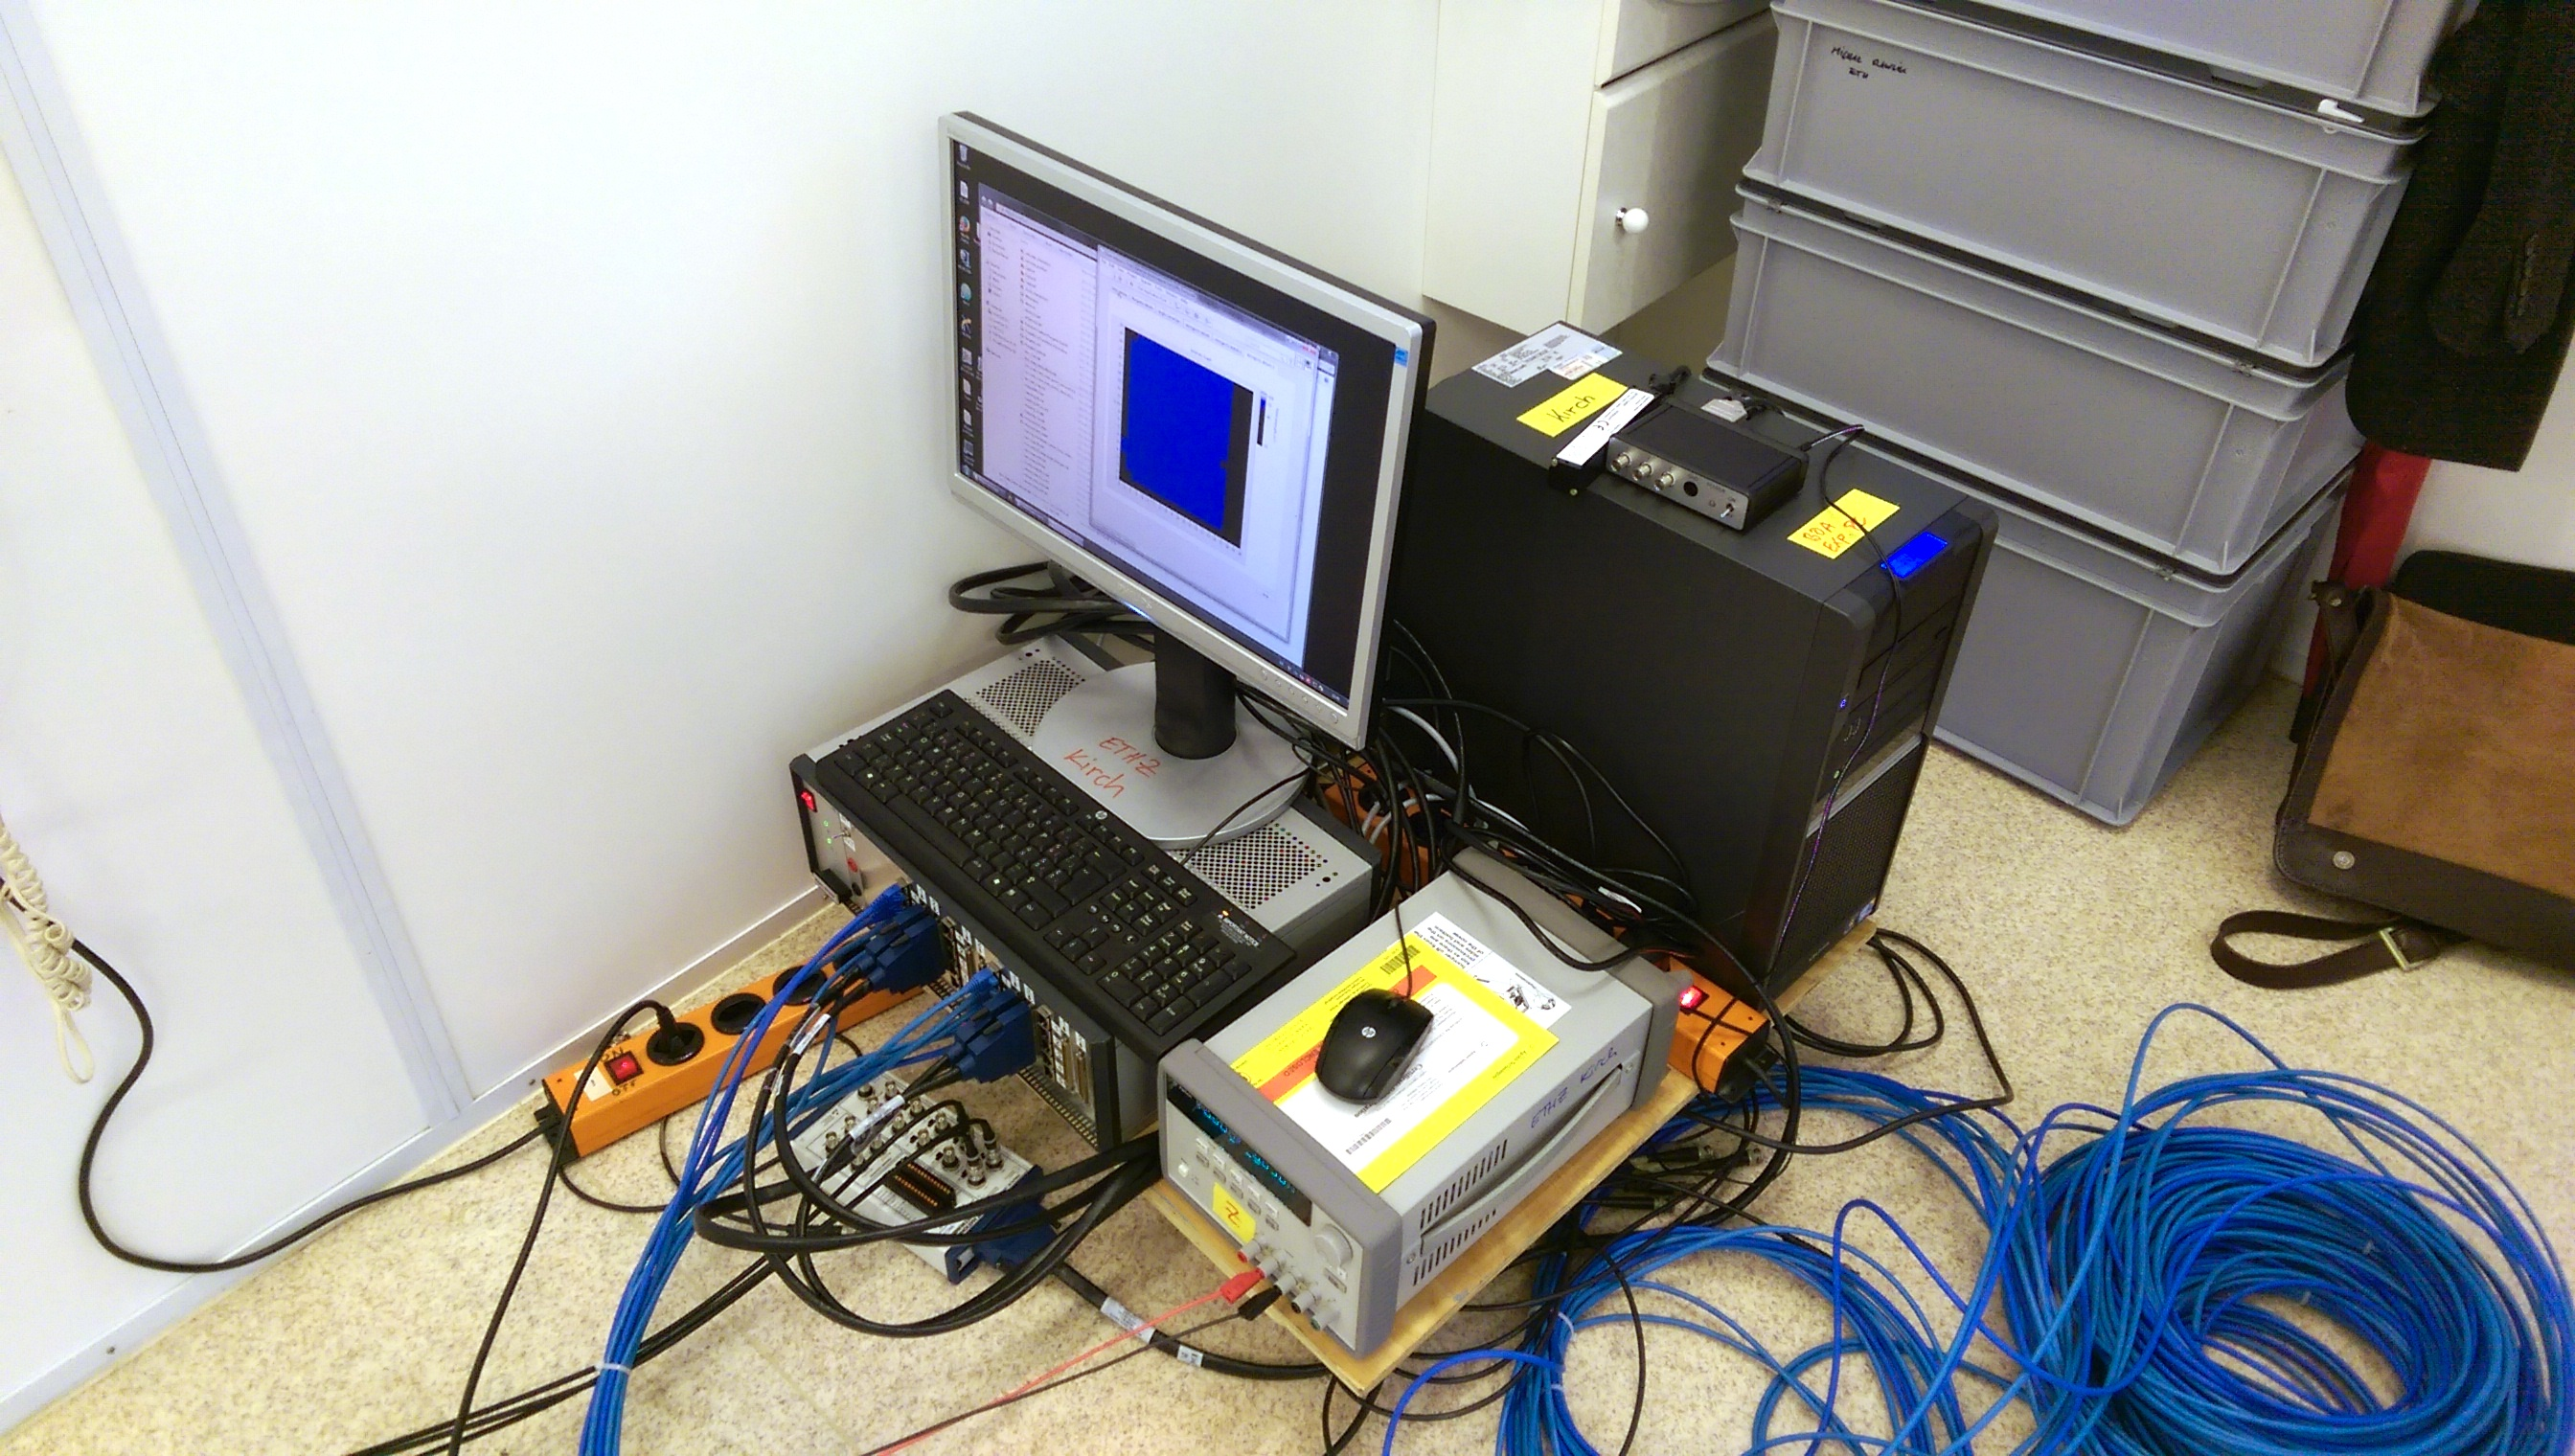
\includegraphics[width=0.9\linewidth]{gfx/mapping/lpsc/daq_edited.jpg}
  \caption{\ldots}
  \label{fig:mapping_bastille_daq}
\end{figure}

The data acquisition system, pictured in Fig.\,\ref{fig:mapping_bastille_daq}, was located on a cart. It consisted of a power supply used to put a constant voltage on the string potentiometers, a custom-built crate for the fluxgates, which supplied them with power and conditioned the incoming signals, and a National Instruments PXI crate, which simultaneously digitised the analogue voltage signals from the fluxgates and the stringpots.

\begin{figure}
  \centering
  \includegraphics[width=\linewidth]{gfx/mapping/lpsc/bastille_panorama_edited.jpg}
  \caption{\ldots}
  \label{fig:mapping_bastille_panorama}
\end{figure}

A panoramic shot of the Bastille room is presented in Fig.\,\ref{fig:mapping_bastille_panorama}. The coordinate system is visible in the upper-left corner. To the right are the entrance door, in the middle a power outlet box is visible.
% Behind the wall with the power outlet box there is a pump, which has been at some point removed.
The room is a wooden structure built in a hall. made of steel beams and sheets. The room's wall with the power outlet is located close, less than 1 metre, to the steel wall of the hall. The hall features a gantry crane, several metres above the roof of the room. On the roof of the room there are air conditioning devices, standing about a metre above the roof on steel legs. The legs have rather large feet, possibly with a steel plate inside.

\begin{figure}
  \centering
  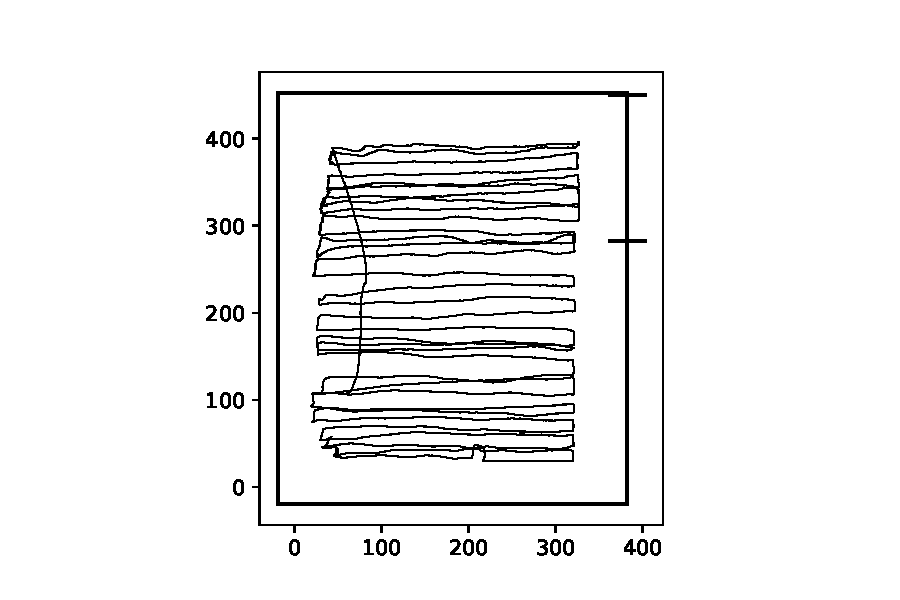
\includegraphics[width=0.9\linewidth]{gfx/mapping/lpsc/bastille_crane_away_rep_track.pdf}
  \caption{\ldots}
  \label{fig:mapping_bastille_track}
\end{figure}

\begin{figure}
  \centering
  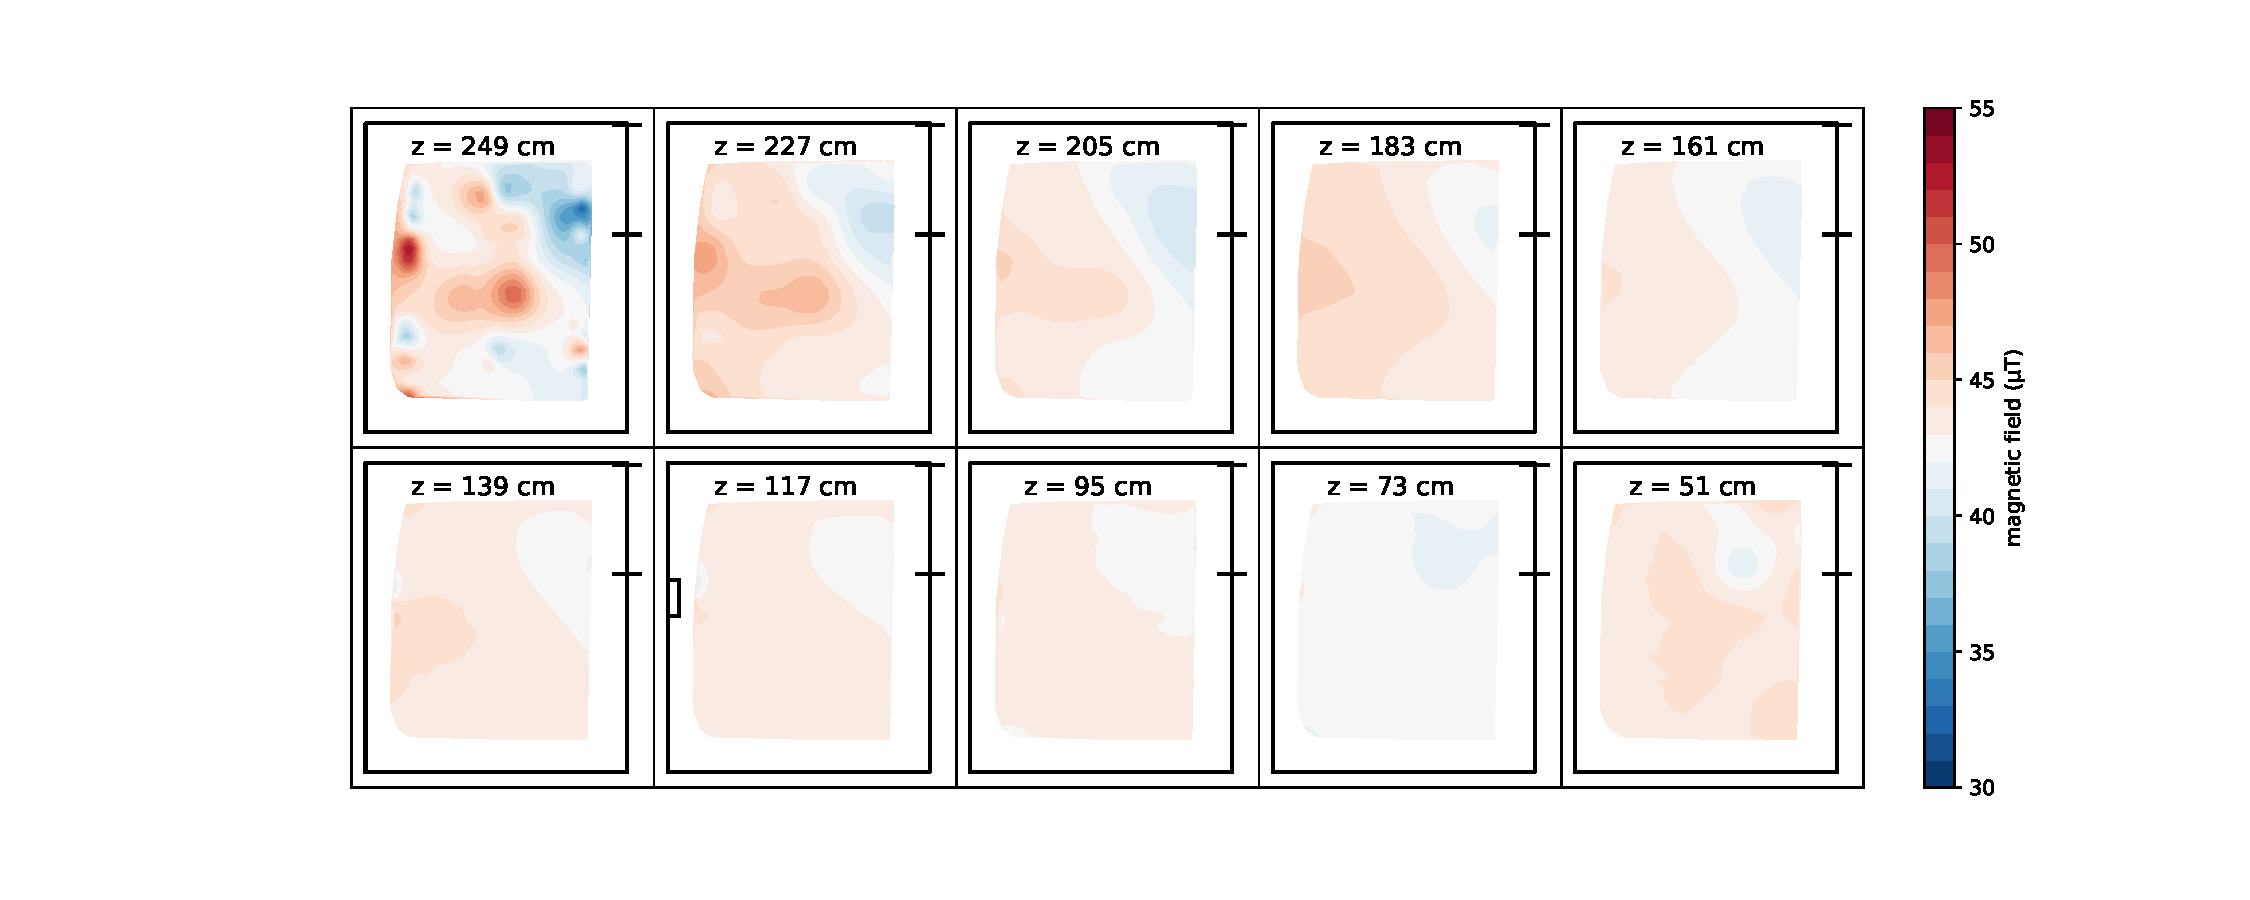
\includegraphics[width=\linewidth]{gfx/mapping/lpsc/bastille_crane_away_rep_magnitude.pdf}
  \caption{\ldots}
  \label{fig:mapping_bastille_magnitude}
\end{figure}

To collect a map, the tower was moved around the room by hand. Care is taken to scan the whole room and to maintain approximately the same orientation of the tower throughout the measurement. The track of one of the collected maps is depicted in Fig\,\ref{fig:mapping_bastille_track}, together with an overview of the room. \note{maybe mention, that the position was calculated on-line, too} Part of the data analysis is performed on-line. In particular the voltage readout of the string pots is translated into their lengths which are used to determine the position and orientation of the tower. This is to provide feedback during the measurements, necessary to make sure that the whole room was scanned. The resulting map was a set of points, collected at \note{give the sampling frequency}, with the position of the tower and magnetic field readout for each fluxgates. Those data are directly plotted in Fig.\,\ref{fig:mapping_bastille_magnitude}. Horizontal slices (each a different sensor) of the magnitude of the magnetic field are shown, with the height of the slice above the floor indicated. It is clearly visible, that there are localised sources of magnetic disturbance above the roof, later attributed to elements of the air-conditioning system mounted on the roof of the hut.

\begin{figure}
  \centering
  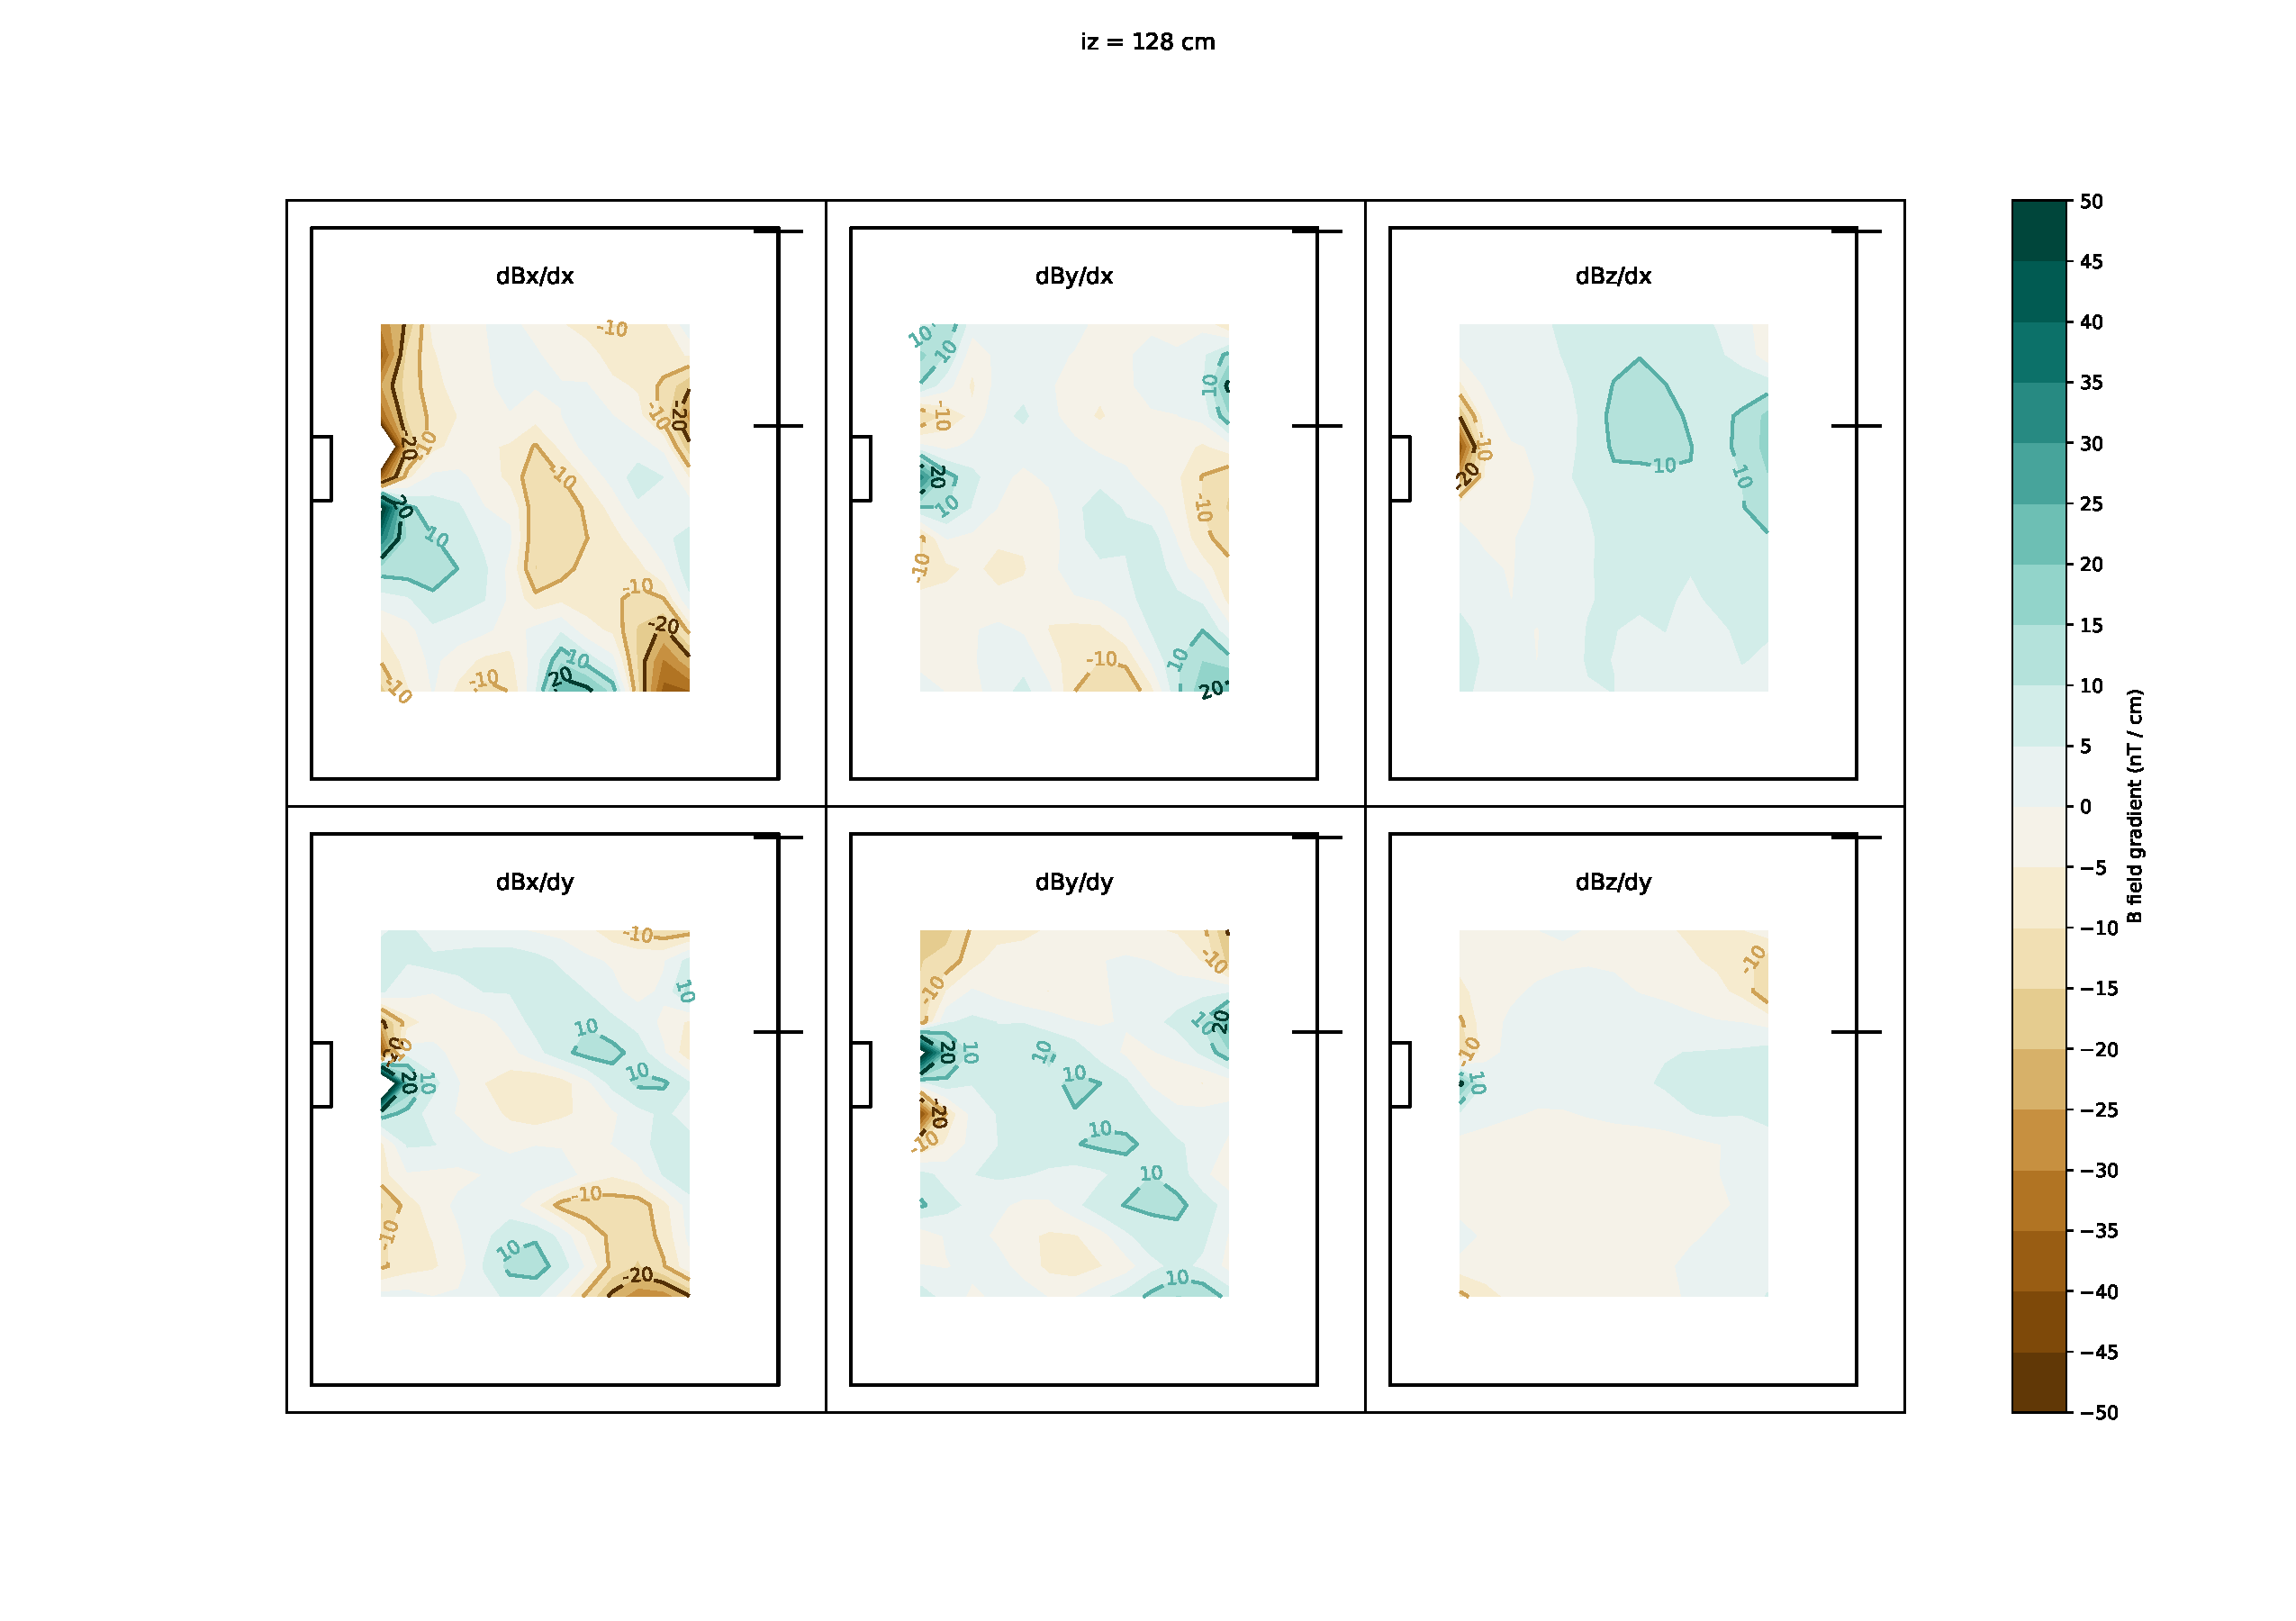
\includegraphics[width=\linewidth]{gfx/mapping/lpsc/bastille_crane_away_rep_gradient_139cm.pdf}
  \caption{\ldots}
  \label{fig:mapping_bastille_gradient}
\end{figure}

The mapper collects not only the magnitude of the field, but the full vector information. This can be used to produce maps of the gradient of the magnetic field. For this purpose the area is divided into pixels, and the average magnetic field is calculated in each.
The the differences between the magnetic field components in the neighbouring pixels are taken, which, divided by the separation between the pixels, are the estimates of the gradient.
For example, the dBx/dx gradient is estimated by the\ldots The map of the gradient \SI{128}{\centi\meter} above the floor is shown in Fig.\,\ref{fig:mapping_bastille_gradient}. Comment on the structures from the roof? On the left side, next to the power outlet box, large gradients above \SI[per-mode=symbol]{20}{\pico\tesla\per\centi\meter} are visible. Only ,,horizontal'' gradients were estimated.
To estimate the vertical ones would require to compare the readouts of different sensors. The sensors are specified to be only $\pm 1\% \pm \SI{0.5}{\micro\tesla}$ accurate, which in a \SI{50}{\micro\tesla} field adds up to \SI{1}{\micro\tesla}. With a \SI{22}{\centi\meter} separation between the sensors, the systematic effect on the gradient would be \SI[per-mode=symbol]{45}{\nano\tesla\per\centi\meter}.

\begin{figure}
  \centering
  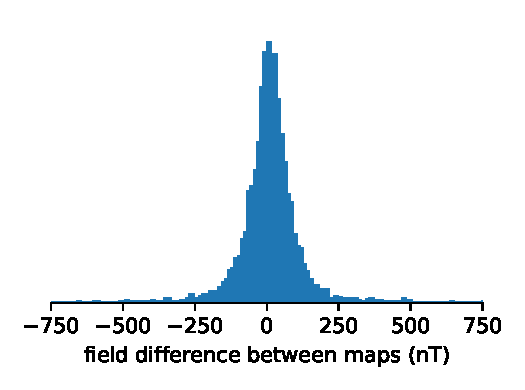
\includegraphics[width=0.8\linewidth]{gfx/mapping/lpsc/reproducibility_field.pdf}
  \caption{\ldots}
  \label{fig:mapping_bastille_reproducibility}
\end{figure}

Binned data allow also for direct comparison between maps. In order to estimate the reproducibility of the mapping process two maps were taken directly one after another. The maps were then, after binning, subtracted from one another. The histogram of the differences is shown in Fig.\,\ref{fig:mapping_bastille_reproducibility} (one entry is one difference in one of the components). The standard deviation of the distribution, a measure of the reproducibility, is \SI{0.14}{\micro\tesla}. The reproducibility of the gradient was estimated in the same way, yielding the standard deviation of \SI[per-mode=symbol]{3.8}{\nano\tesla\per\centi\meter}. This is better than a na\"{\i}ve estimate, which assumes that the value of the component of the field measured in one bin has a \SI{0.14}{\micro\tesla} uncorrelated error bar associated with it:
\begin{equation}
  \frac{\SI{140}{\nano\tesla} \, \sqrt{2}}{\SI{25}{\centi\meter}} = \SI[per-mode=symbol]{8}{\nano\tesla\per\centi\meter} \ .
\end{equation}
The reason is, that the for the absolute field estimate to be reproducible the system needs to be stable on a large scale -- from one map to another. For the gradient of the field to be reproducible, the system needs to be stable only from one bin to the next.

\begin{figure}
  \centering
  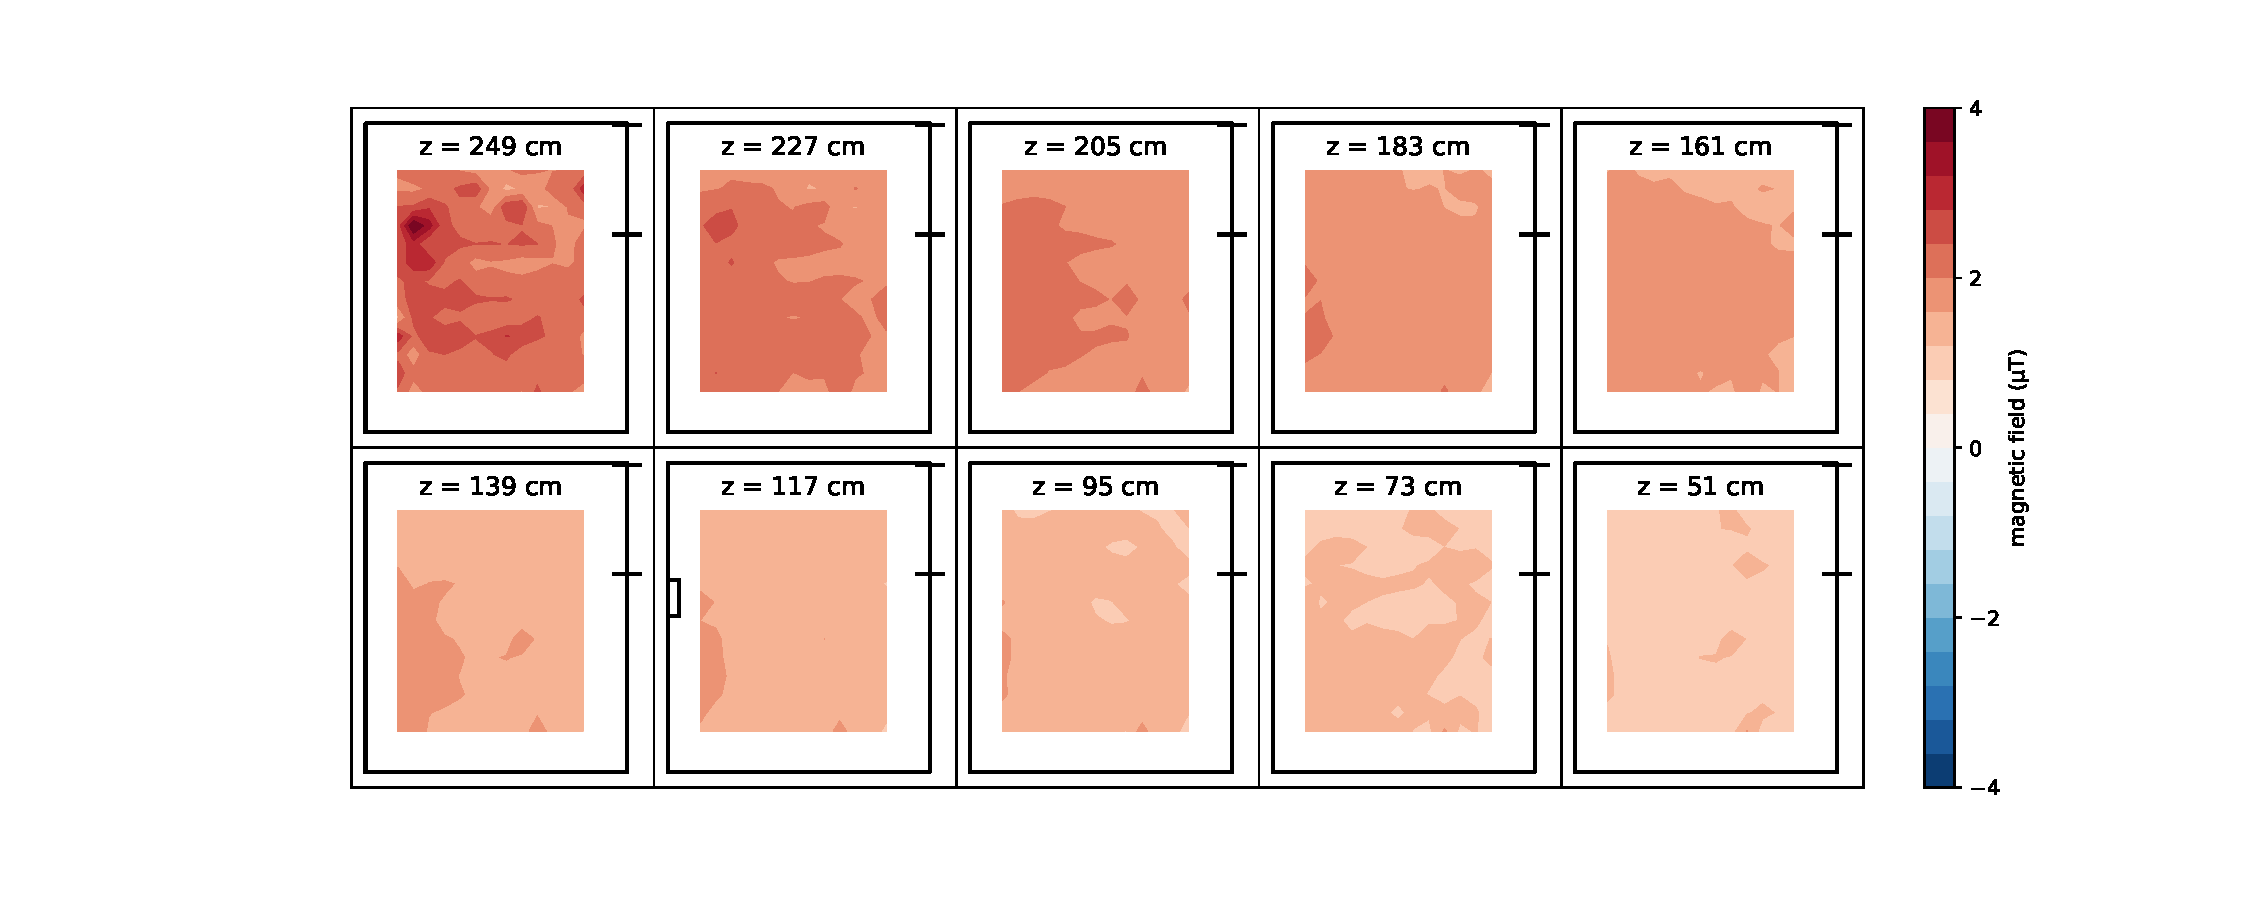
\includegraphics[width=\linewidth]{gfx/mapping/lpsc/bastille_crane_change_magnitude.pdf}
  \caption{\ldots}
  \label{fig:mapping_bastille_crane_change}
\end{figure}

The reproducibility of the gradient esti

First the reproducibility, then a differential map.


Several maps were performed. 


First the setting. Magnetic characterisation of a new laboratory room, designated for Hg-199 magnetometry research.
A picture of the room (and the mapper, too?).

The setup is shown\ldots The mapper was a tower this and that high, with ten fluxgate magnetometers mounted on it.
The three analogue string potentiometers were mounted on a rigid L-piece (give the positions).
\marginpar{A string potentiometer has a spring-loaded spool attached to a potentiometer. For maximal linearity it is constructed in a way, that the string is wound one layer only.}

Naively estimated the error on the measurement in a bin is 140nT, so for a gradient it is 140nT∗2√25cm=8 nT/cm. It is, however, better in reality - 3.8 nT/cm. To have a good estimate on the gradient the system needs to be stable and reproducible on small scales (25cm and less then a second). For the absolute field measurement to be reproducible the whole system needs to be stable on scales of 400cm and half and hour.



% \begin{figure}
%   \centering
%   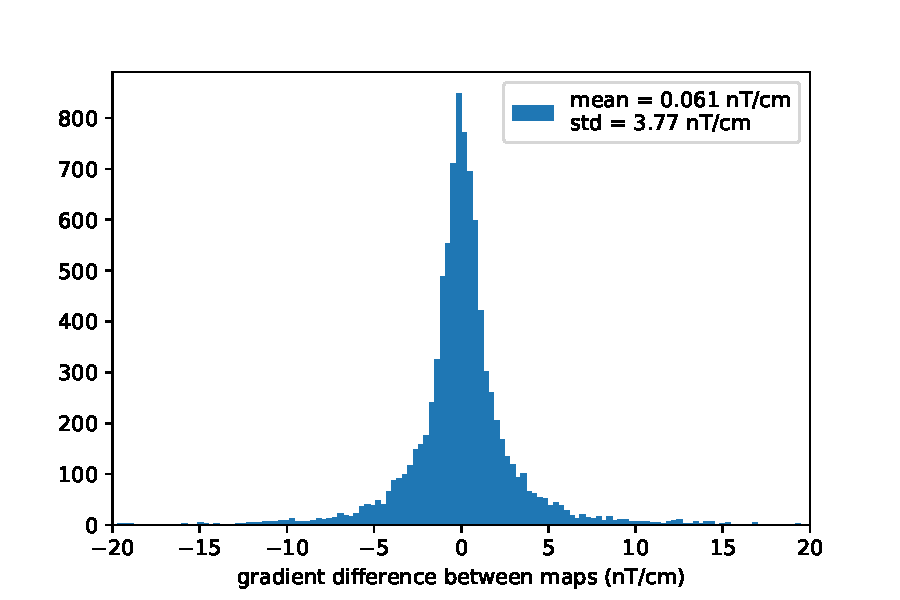
\includegraphics[width=0.8\linewidth]{gfx/mapping/lpsc/reproducibility_gradient.pdf}
%   \caption{\ldots}
%   \label{fig:mapping_bastille_magnitude}
% \end{figure}




\section{PSI Area South campaign}

Acknowledge that it is a joint work with Solange Emmenegger.

Describe the changes to the setup: now the geometry is like this and this. Need probably a detailed picture of the geometry of the setup and the mapper.

About the method to fit the calibration parameters to the fixed points.